%Setup the document style and format
\documentclass[a4paper,10pt]{article}

\usepackage{geometry}
\geometry{
	a4paper,
	total={170mm,240mm},
	left=20mm,
	top=30mm,}

%Import packages 
\usepackage{caption}
\usepackage{appendix}
\usepackage{natbib}
\usepackage{float}
\usepackage{graphics}
\usepackage{graphicx}
\usepackage{multirow}
\usepackage{etoolbox}
\usepackage{amsmath,amsfonts,amsthm}
\usepackage[siunitx,american,arrowmos]{circuitikz}
\usepackage{titling}
\usepackage{amsmath,amsfonts,amsthm}
\usepackage[siunitx,american,arrowmos]{circuitikz}

%Setup for inline code listings
\usepackage{listings}
\usepackage{xcolor}
\definecolor{codegreen}{rgb}{0,0.6,0}
\definecolor{codegray}{rgb}{0.5,0.5,0.5}
\definecolor{codepurple}{rgb}{0.58,0,0.82}
\definecolor{backcolour}{rgb}{0.95,0.95,0.92}
\lstdefinestyle{mystyle}{
    language=Java,
    backgroundcolor=\color{backcolour},   
    commentstyle=\color{codegray},
    keywordstyle=\color{orange},
    numberstyle=\tiny\color{codegray},
    stringstyle=\color{codegreen},
    basicstyle=\ttfamily\small,
    breakatwhitespace=false,         
    breaklines=true,                 
    captionpos=b,                    
    keepspaces=true, 
    numbers=left,                 
    numbersep=5pt,                  
    showspaces=false,                
    showstringspaces=false,
    showtabs=false,                  
    tabsize=2
}
\lstset{style=mystyle}

\begin{document}

\begin{titlepage}


\newcommand{\HRule}{\rule{\linewidth}{0.5mm}}
\center
\vspace*{4cm}
\textit{\Large Sample Latex Document}
\HRule\\[0.4cm]
{\huge\bfseries Title 1\vspace*{10mm} \\Title 2\\[0.4cm]
\HRule\\[1.5cm]
{\large\textit{Author}}\\
 \textsc{T.Phelan}\\
\vfill\vfill\vfill
{\large 2022}
\vfill}

\tableofcontents
\end{titlepage}

\section{Text and Tables}

\subsection{Text Formatting}
\paragraph{} The document is written in \textbf{whichever} \textit{formatting} \texttt{is appropriate}. It can be broken into sections, subsections, subsubsections paragraphs, and make reference to included images, graphics, math, equations, code and bibliography.

\subsubsection{Lorem Ipsum}
\paragraph{}Lorem ipsum dolor sit amet, consectetur adipiscing elit, sed do eiusmod tempor incididunt ut labore et dolore magna aliqua. Cursus eget nunc scelerisque viverra mauris in aliquam sem. Blandit volutpat maecenas volutpat blandit aliquam etiam erat. Etiam sit amet nisl purus in mollis nunc sed id. Consequat interdum varius sit amet mattis vulputate enim. Non curabitur gravida arcu ac tortor dignissim convallis. Facilisi etiam dignissim diam quis enim lobortis scelerisque. Purus semper eget duis at tellus at urna. Vel pharetra vel turpis nunc eget lorem dolor sed. Vestibulum rhoncus est pellentesque elit. Ultricies leo integer malesuada nunc vel risus commodo viverra. Dui sapien eget mi proin sed. Adipiscing vitae proin sagittis nisl rhoncus mattis rhoncus urna.

\subsection{Tabular Formatting}
\paragraph{} We can represent data in a tabular format, as in Table~\ref{table}.

\subsubsection{Table}
\begin{table}[!h]
\centering
	\begin{tabular}{|c|c|c|}
	\hline
    \textbf{Hours}& \textbf{Minutes}& \textbf{Seconds} \\ \hline
           0      &         0       &         0        \\ \hline
           1      &         60      &       3600       \\ \hline
           2      &        120      &       7200       \\ \hline
           24     &        1440     &       86400      \\ \hline
 
	\end{tabular}
	\caption{\textit{An example of a simple table}}
	\label{table}
\end{table}

\section{Mathematical Formatting}\label{math}
\subsection{In-line Mathematics}
Math formulas can appear in line in text such as $y= \dfrac{m}{x}+b$ or be referenced as a standalone equation, such as Eq.~\eqref{eq1} and Eq.~\eqref{eq2}.

\subsection{Some Equations}
	\begin{equation}\label{eq1}
	I_D = I_S \left[\exp\left(\dfrac{V_D}{V_T}\right)-1\right]
	\end{equation}
	\begin{equation}\label{eq2}
	V_D = v_s - V_R
	\end{equation}

\newpage

\section{Graphics and Diagrams}

\paragraph{} Figure~\ref{fig:Circuit} is a wiring digram of a simple resistive circuit with a diode. Eq.~\eqref{eq1} and Eq.~\eqref{eq2} are theoretical mathematical formulas for the expected quantities one would measure in the circuit.\\
Figure~\ref{plot} shows a graphical plot of the theoretical equations \eqref{eq1} and \eqref{eq2} as applicable to the circuit in figure~\ref{fig:Circuit}.

\subsection{Circuit Diagram}

\begin{figure}[ht]\centering
	\begin{circuitikz}[scale=1, transform shape]
		\draw
		(0,0)  to [V,V_=$v_s$,-*] ++(0,-3) node[ground](g){}
		
		(0,0) to [short] ++(1,0) 
		to [R, l=$R$] ++(2,0) 
		to [short,i=$I_D$] ++(1,0) 
		to [D, v^=$V_D$] ++(0,-3) 
		to (g)
		;
	\end{circuitikz}
	\caption{\textit{A Circuitikz Diagram.}}
	\label{fig:Circuit}
\end{figure}

\subsection{Graphics}

\begin{figure}[!h]
	\centering
	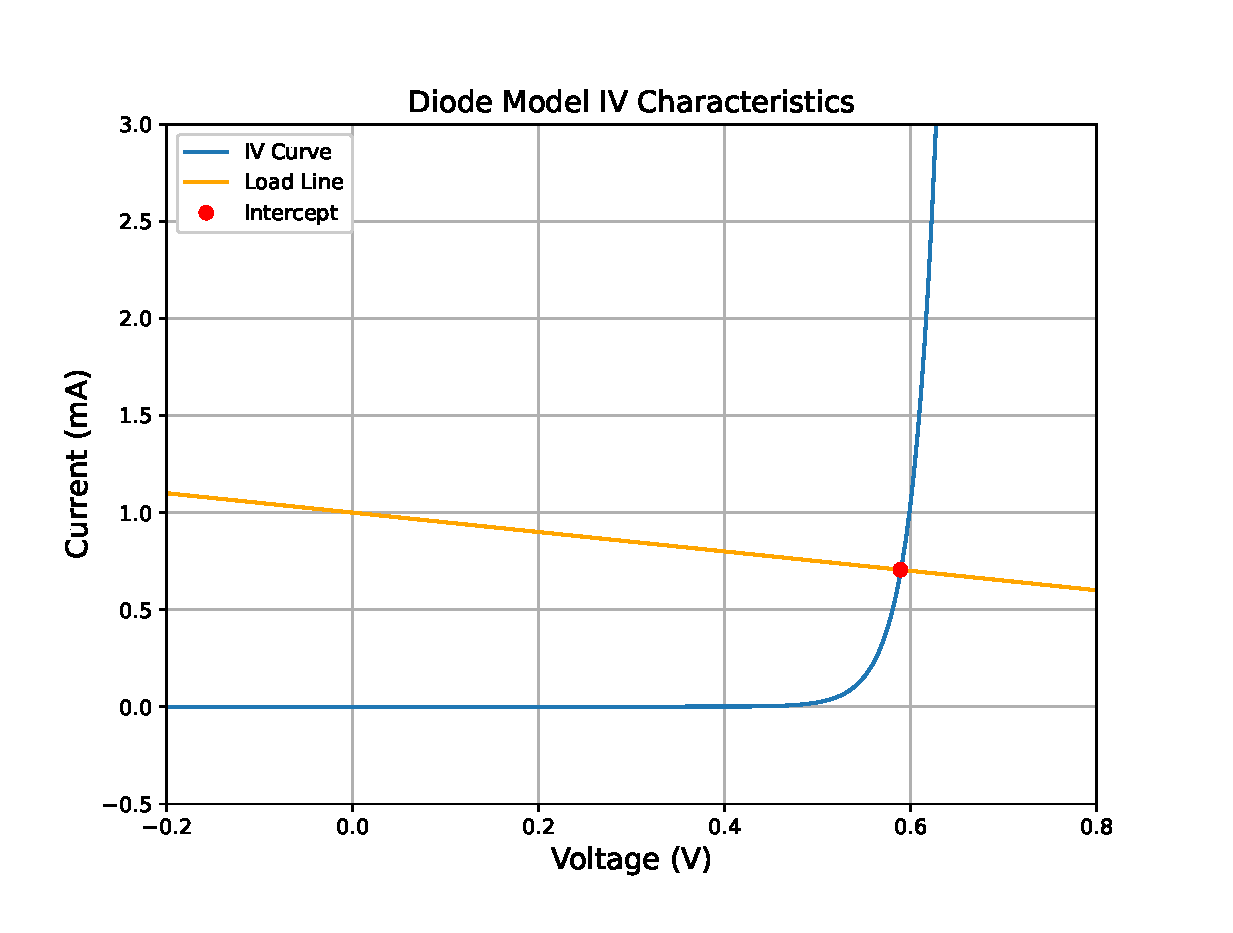
\includegraphics[width=250px]{plot.eps}
	\caption{\textit{Graphical representation of the Diode model.}}
	\label{plot}
\end{figure}

\newpage
\section{Code Listings}\label{code}
\subsection{}Verbatim code listings can be directly represented with appropriate syntax highlighting applied for whichever programming language is being represented. Figure~\ref{java} is a code listing of a generic Java class.

\subsection{SampleClass.java}
\begin{figure}[!h]
	\begin{lstlisting}
public class SampleClass extends Object implements Comparable<T>{
    
    int var1;
    String msg;
    
    SampleClass(String msg){
        super();
        this.msg = msg;
    }
    @Override
    public int compareTo(T o) {
        return 0;
    }
    @Override
    public String toString() {
        return "SampleClass{" +
                "msg='" + msg + '\'' +
                '}';
    }
}
	\end{lstlisting}
	\caption{\textit{SampleClass.java}}
	\label{java}
\end{figure}

\end{document}
